\subsection{Schermata risultati test}
Schermata che mostra tutti i dati relativi al test salvato o appena eseguito.

\begin{figure}
\centering
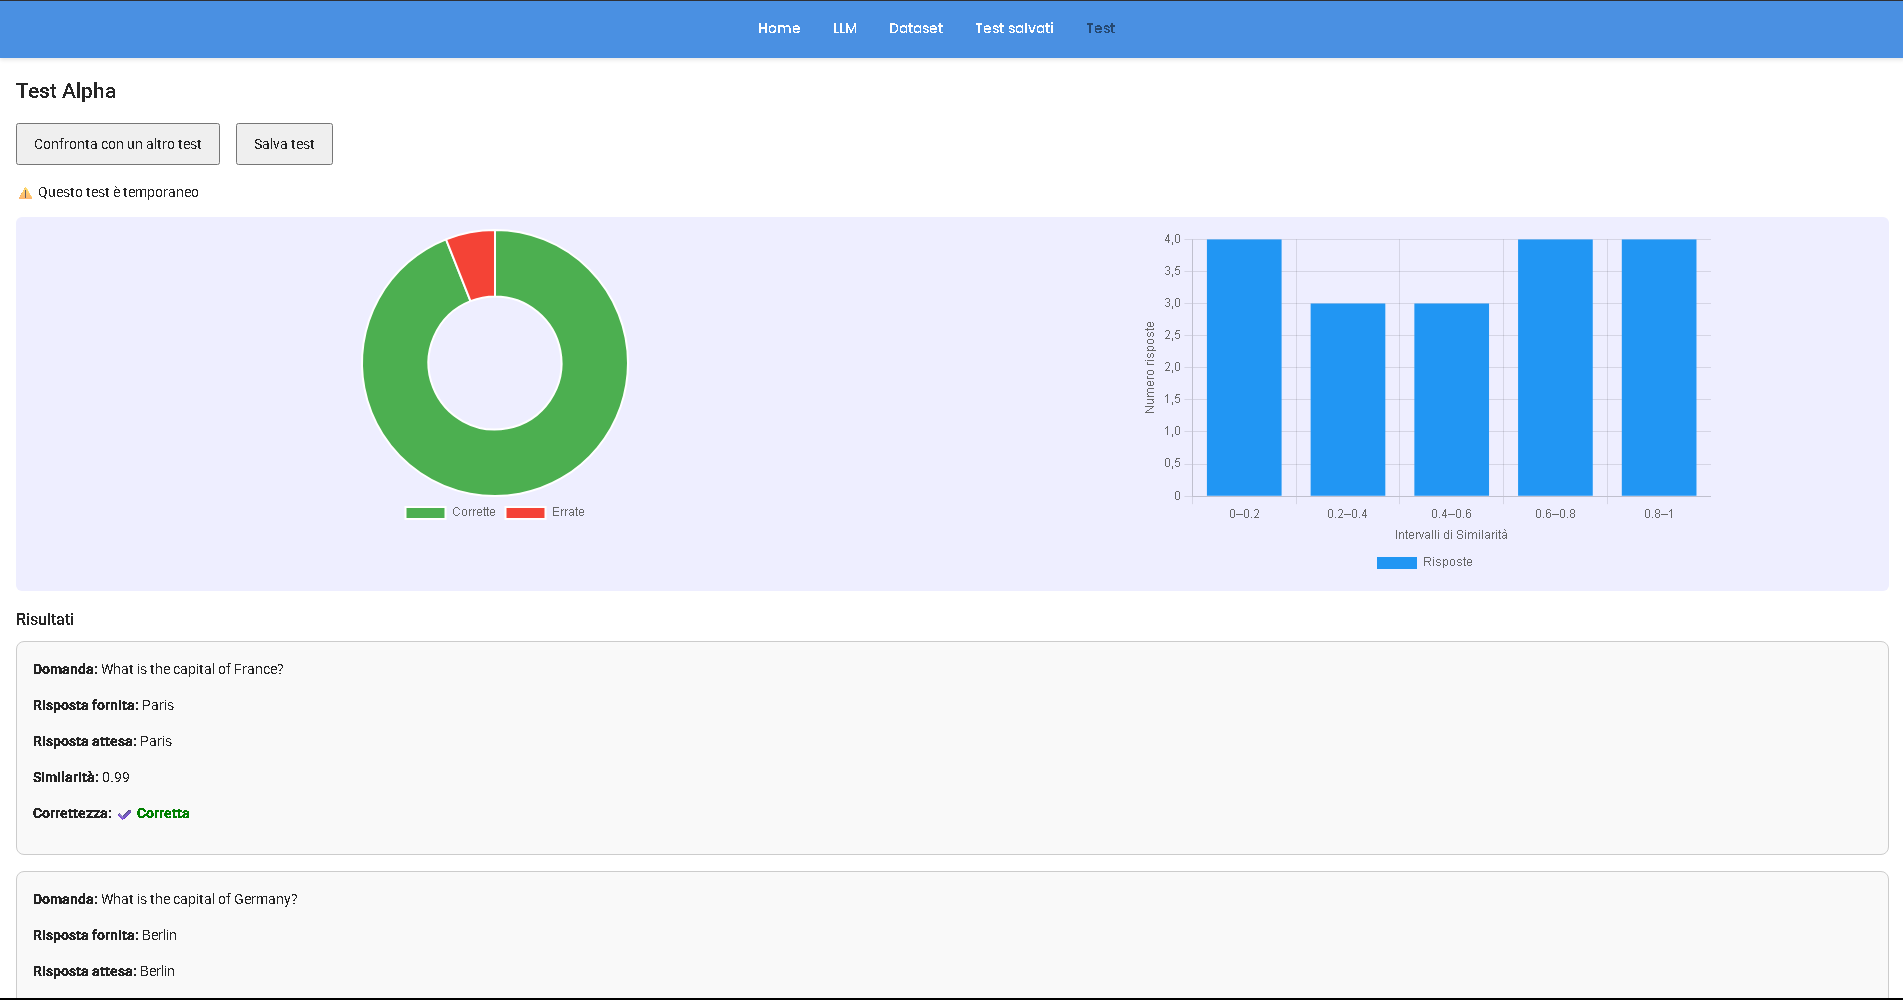
\includegraphics[width=0.25\linewidth]{Immagini/Test.png}
\caption{\label{fig:risultati_test}Schermata per la visione dei risultati di un test.}
\end{figure}

\subsubsection{Confronto dei test}
Consente di confrontare due test tramite una scrollview con i test salvati.
\begin{figure}
\centering
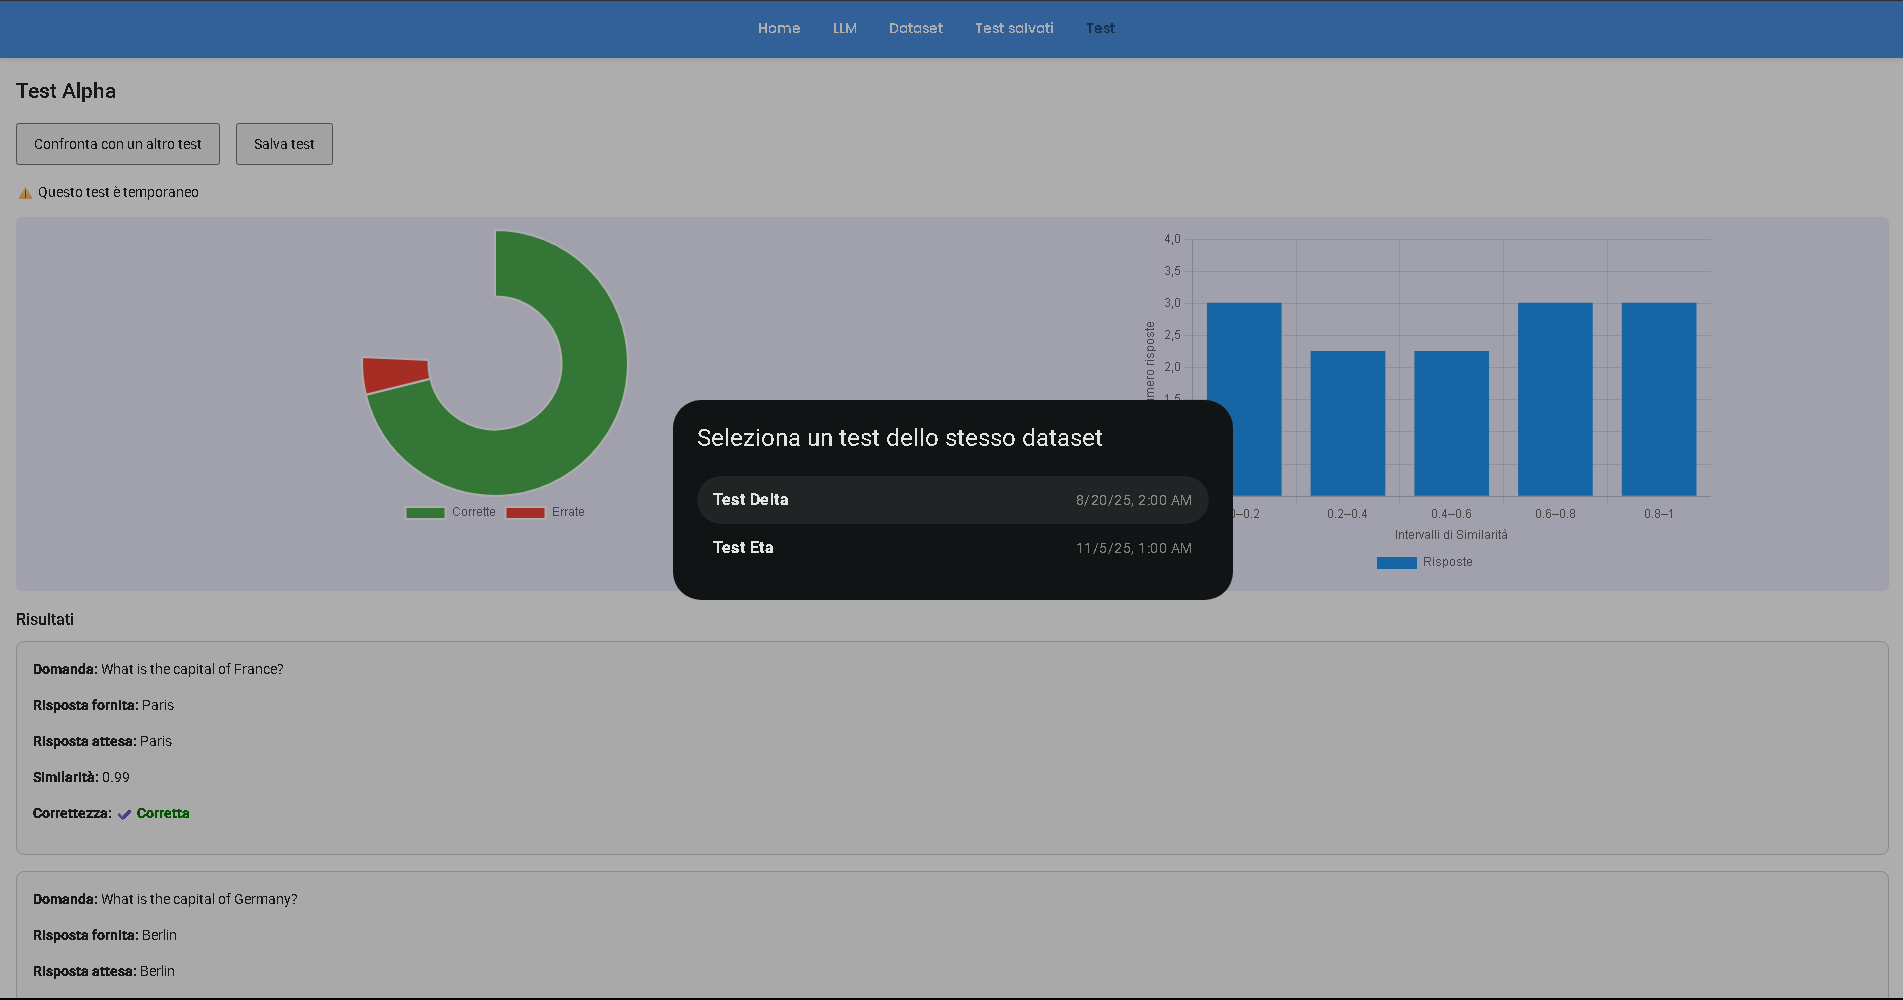
\includegraphics[width=0.25\linewidth]{Immagini/Choose_Test_Option.png}
\caption{\label{fig:confronto_test}Opzione per il confronto dei test.}
\end{figure}

\subsubsection{Rinominazione di un test}
Consente di rinominare il test mostrando un form per l'inserimento del nuovo nome.
\begin{figure}
\centering
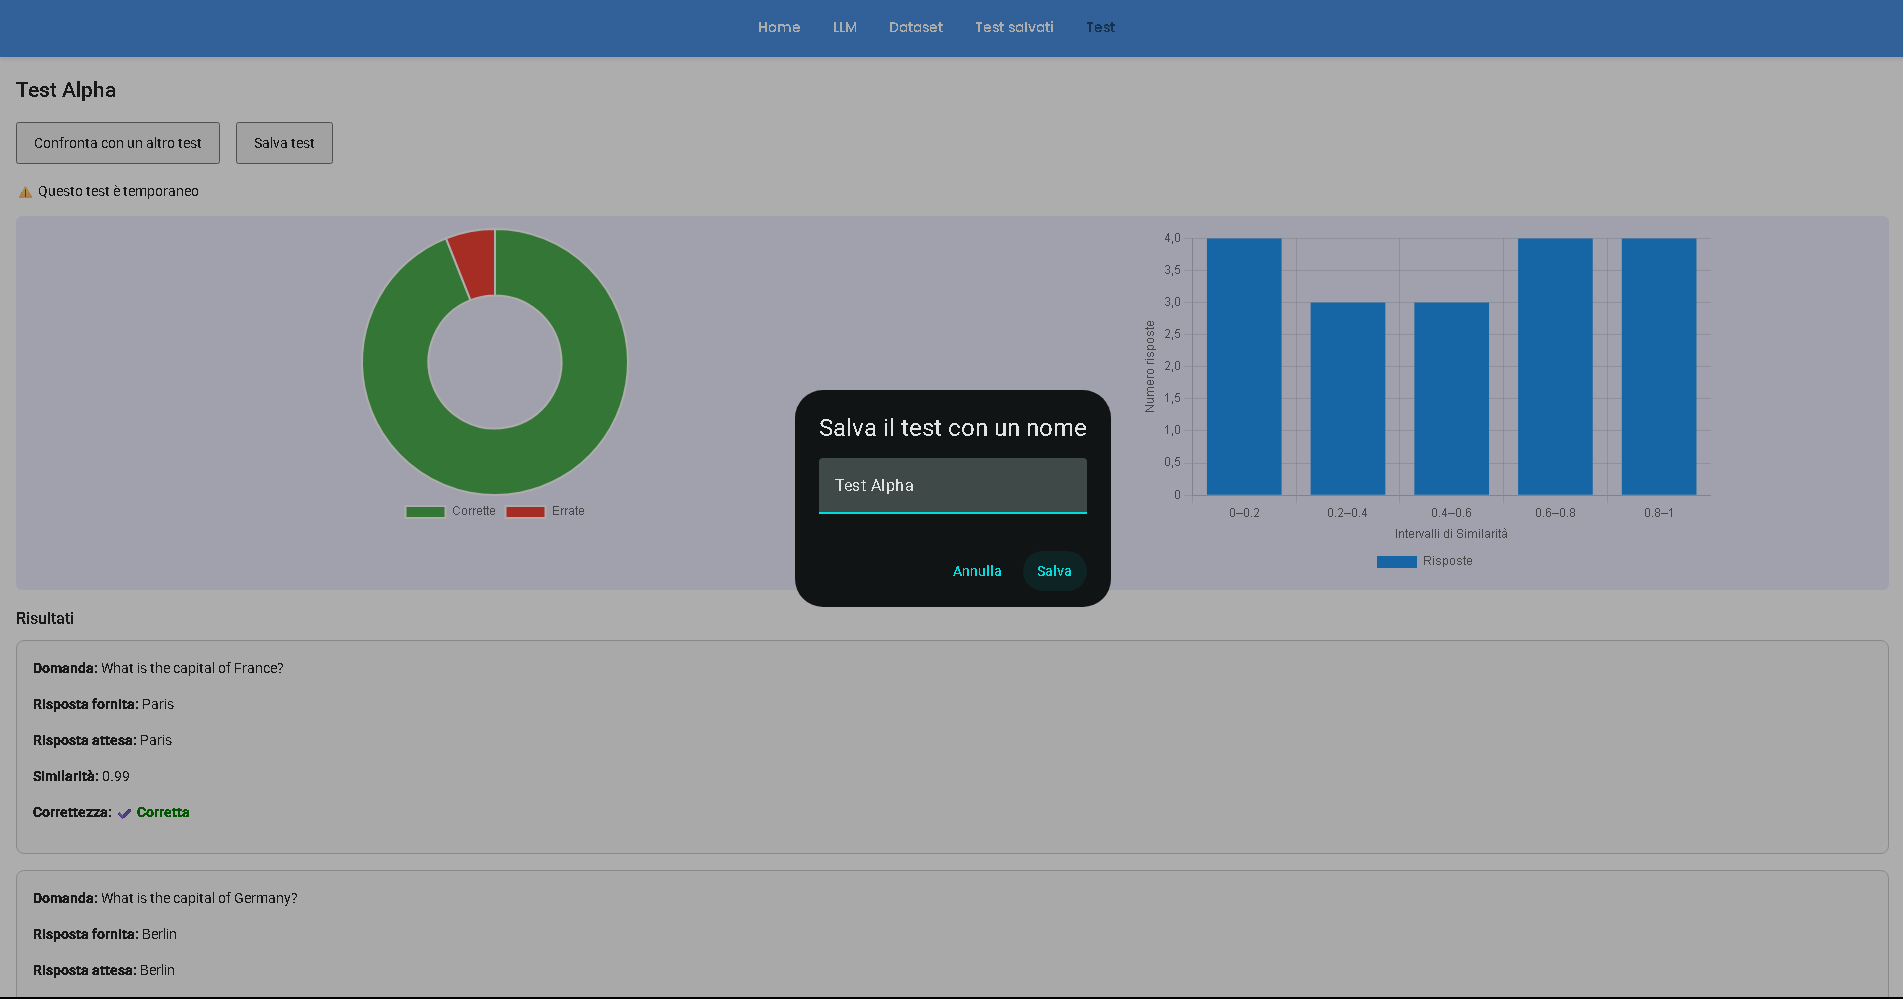
\includegraphics[width=0.25\linewidth]{Immagini/Rename_Test_Option_2.png}
\caption{\label{fig:rinomina_test_2}Opzione per il cambio di nome al test.}
\end{figure}

\subsubsection{Scatter Plot}
Mostra i valori di similarità delle risposte dell LLM rispetto le risposte reali attese.
\begin{figure}
\centering
\includegraphics[width=0.25\linewidth]{Immagini/Scattter_Test.png}
\caption{\label{fig:scatter_test}Schermata per lo scatter plot del test.}
\end{figure}